\section{\emph{Depth Camera}}
\label{sec:depthcamera}

\emph{Depth camera} merupakan salah satu jenis kamera yang dapat digunakan untuk menghasilkan citra dua dimensi yang menampilkan jarak suatu titik dari pusat kamera.
Terdapat berbagai metode yang dapat digunakan untuk menghasilkan citra kedalaman (\emph{depth image}) dari sebuah \emph{depth camera},
  salah satunya adalah dengan menangkap pantulan cahaya menggunakan sistem \emph{time of flight} \citep{cit:idan2001}.
Seperti yang terlihat pada gambar \ref{fig:diagramtimeofflight},
  kamera dengan sistem tersebut akan memancarkan cahaya dan mengukur waktu tempuh dari pantulan cahaya tersebut ketika tertangkap kembali oleh kamera.

\begin{figure}[ht]
  \centering
  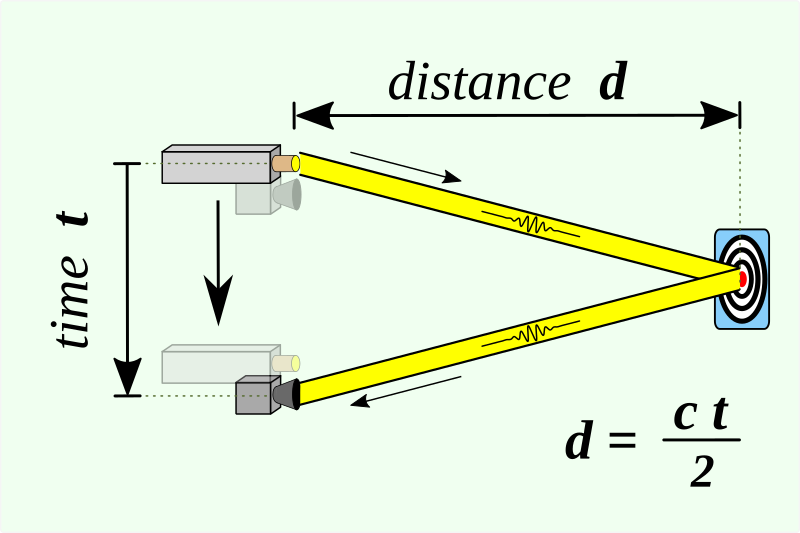
\includegraphics[scale=0.2]{gambar/diagram-time-of-flight.png}
  \caption{Diagram cara kerja sistem \emph{time of flight} \citep{url:timeofflight}.}
  \label{fig:diagramtimeofflight}
\end{figure}

Selain cara tersebut,
  citra kedalaman juga dapat diperoleh dengan cara melakukan perhitungan triangulasi pada dua atau lebih citra yang dihasilkan oleh sistem multi-kamera.
Jarak suatu titik pada kamera dengan sistem ini dapat dihitung dengan melakukan korespondensi pada citra-citra yang dihasilkan.
Berbeda dengan metode sebelumnya,
  \emph{depth camera} dengan metode ini memiliki keunggulan dimana estimasi yang didapatkan bersifat kurang lebih pasif,
  dimana estimasi tersebut tidak banyak dipengaruhi oleh kondisi pencahayaan yang ada pada lingkungan.

\subimport{7-depth-camera}{1-kinect-v2.tex}
\subimport{7-depth-camera}{2-libfreenect2.tex}
